% Team report, following the course template (references/mlops_report_template.md).
% Build with `make report` (draft) or `make report-submit` (see reports/latex/README.md).
\documentclass[11pt, a4paper]{article}
% Shared preamble for report.tex and edn.tex.

% --- Build flags ------------------------------------------------------------
% Set from the command line by the Makefile (latexmk -usepretex), so a plain
% compile in an editor gives the defaults: initial report, guidance visible.
%   \ReportFinal       final report (Milestones 1-6) instead of initial (1-3)
%   \ReportSubmission  hide guidance boxes and example content
\newif\iffinalreport
\ifdefined\ReportFinal \finalreporttrue \fi
\newif\ifguidance
\guidancetrue
\ifdefined\ReportSubmission \guidancefalse \fi

% --- Packages ---------------------------------------------------------------
\usepackage[T1]{fontenc}
\usepackage[utf8]{inputenc}
\usepackage{lmodern}
\usepackage[english]{babel}
\usepackage{microtype}
% `--` inside \texttt stays two hyphens instead of the en dash the T1 ligature makes,
% so command-line options such as `ruff format --check` print as typed.
\DisableLigatures[-]{encoding=T1,family=tt*}
% Typewriter text gets no extra space after a colon or a full stop, so `push: false`
% prints with one space as typed and not two.
\AddToHook{ttfamily}{\frenchspacing}
\usepackage[a4paper, margin=2.5cm, headheight=14pt]{geometry}
\usepackage{graphicx}
\graphicspath{{figures/}{../figures/}}
\usepackage[table]{xcolor}
\usepackage{booktabs}
\usepackage{tabularx}
\usepackage{array}
\usepackage{amssymb}
\usepackage{enumitem}
\usepackage{etoolbox}
\usepackage{fancyhdr}
\usepackage{listings}
\usepackage[most]{tcolorbox}
\usepackage{csquotes}
\usepackage[backend=biber, style=ieee]{biblatex}
\addbibresource{references.bib}
% Let long URLs in the bibliography break anywhere instead of overflowing.
\setcounter{biburlnumpenalty}{9000}
\setcounter{biburllcpenalty}{7000}
\setcounter{biburlucpenalty}{8000}
\usepackage[hidelinks]{hyperref}
\usepackage[capitalise, noabbrev]{cleveref}

% Team and project facts shown on the cover pages. Edit here, nowhere else.
% Replace every \tbd{...} before a submission.

\newcommand{\TeamName}{Recommenditos}
\newcommand{\ProjectTitle}{Car price estimation ML system}
\newcommand{\CourseName}{Machine Learning Systems in Production (MLOps)}
\newcommand{\CourseProgram}{Master in Data Science, Universitat Polit\`ecnica de Catalunya (UPC)}
\newcommand{\CourseTerm}{2026/27 Q1}

% Links (course rules: GitHub repo plus any other resources we use).
% Shown without the https:// prefix so they fit on one line.
\newcommand{\RepoLink}{\href{https://github.com/mlops-2627q1-mds-upc/MLOPS_Recommenditos}{\nolinkurl{github.com/mlops-2627q1-mds-upc/MLOPS_Recommenditos}}}
\newcommand{\BoardLink}{\href{https://github.com/orgs/mlops-2627q1-mds-upc/projects/1}{\nolinkurl{github.com/orgs/mlops-2627q1-mds-upc/projects/1}}}
\newcommand{\DiscordLink}{Discord (team channel, invite on request)}
\newcommand{\DagsHubLink}{\href{https://dagshub.com/recommenditos/MLOPS_Recommenditos}{\nolinkurl{dagshub.com/recommenditos/MLOPS_Recommenditos}}}
\newcommand{\SlidesLink}{\href{https://docs.google.com/presentation/d/1XdgoTZ3ld9GcNNu0bmRhdAA0rSdVDUgLxD-ssI6hk70/edit}{\nolinkurl{docs.google.com/presentation/d/1XdgoTZ3ld9GcNNu0bmRhdAA0rSdVDUgLxD-ssI6hk70}}}
\newcommand{\ApiLink}{\tbd{deployed API URL}}

% One address that reaches the whole team (course rule). We have no shared
% mailing list, so this is the Scrum Master, who forwards to the team.
\newcommand{\TeamMail}[1]{\href{mailto:#1}{\nolinkurl{#1}}}
\newcommand{\TeamContact}{\TeamMail{lukas.haeussler@estudiantat.upc.edu} (Scrum Master, forwards to the whole team)}

% Team members, used on the cover page and in the CATME table.
% Short names are what appears in the CATME table headers.
\newcommand{\MemberA}{Lukas}
\newcommand{\MemberB}{Kevin}
\newcommand{\MemberC}{Urszula}
\newcommand{\MemberD}{Michal}
\newcommand{\MemberE}{Mark}

% Rows for the cover page table: Surname & Name & UPC e-mail & GitHub account.
% Addresses exactly as recorded in the repository README. Mark's is on
% estudiant.upc.edu, the other four are on estudiantat.upc.edu.
\newcommand{\TeamMemberRows}{%
  H\"au{\ss}ler & Lukas & \TeamMail{lukas.haeussler@estudiantat.upc.edu} & \texttt{lukas2510} \\
  Adameit & Kevin & \TeamMail{kevin.adameit@estudiantat.upc.edu} & \texttt{kadameit} \\
  Sawczuk & Urszula & \TeamMail{urszula.wanda.sawczuk@estudiantat.upc.edu} & \texttt{ulasawczuk} \\
  Dudek & Michal & \TeamMail{michal.feliks.dudek@estudiantat.upc.edu} & \texttt{michudud04} \\
  Atzberger & Mark & \TeamMail{mark.welf.atzberger@estudiant.upc.edu} & \texttt{W11W11W11} \\
}


\hypersetup{
  pdftitle={MLOps\_\TeamName},
  pdfauthor={Team \TeamName},
}

\setlist{itemsep=2pt, topsep=4pt}
\setlength{\parindent}{0pt}
\setlength{\parskip}{0.5em}

\lstset{
  basicstyle=\ttfamily\small,
  breaklines=true,
  frame=single,
  columns=fullflexible,
}

\pagestyle{fancy}
\fancyhf{}
\renewcommand{\headrulewidth}{0.4pt}
\fancyfoot[C]{\thepage}

% --- Writing helpers --------------------------------------------------------

% \guidance{...}: what a section should contain, taken from the course
% template, the lab rubric and the demo repo. Hidden in submission builds.
\newtcolorbox{guidancebox}{
  breakable, colback=blue!4, colframe=blue!45!black, boxrule=0.5pt,
  fonttitle=\small\bfseries, title={Guidance (hidden in submission build)},
  fontupper=\small, left=4pt, right=4pt, top=2pt, bottom=2pt,
}
\newcommand{\guidance}[1]{\ifguidance\begin{guidancebox}#1\end{guidancebox}\fi}

% \tbd{...}: a placeholder that still has to be filled in. Always rendered in
% red, and counted by `make report-submit` so nothing slips into a submission.
\newcommand{\tbd}[1]{%
  \GenericWarning{}{Report warning: Unfilled placeholder: #1}%
  \textcolor{red}{\textbf{[TBD: #1]}}%
}

% Course repositories and documents we refer to.
\newcommand{\demorepo}{\url{https://github.com/mlops-2627q1-mds-upc/MLOps-2627q1-demos}}


\iffinalreport
  \newcommand{\Deliverable}{Final report (Milestones 1--6)}
\else
  \newcommand{\Deliverable}{Initial report (Milestones 1--3)}
\fi

\fancyhead[L]{\small MLOps\_\TeamName}
\fancyhead[R]{\small \Deliverable}

\setcounter{tocdepth}{2}

% The EDN is appended as built (Atenea takes one PDF). build.sh builds it first
% and names its job here; a plain compile in an editor takes the draft.
\usepackage{pdfpages}
\providecommand{\EdnJob}{edn}

% \appendixpdf{title}{file}{label} appends a PDF as the next appendix: it takes
% the next letter, gets a line in the contents and a bookmark, and is listed on
% the divider page, which \appendixdivider prints from the .apx file, the way
% \tableofcontents prints from the .toc file.
\makeatletter
\newcounter{apxpageoffset}
\newcommand{\appendixpdf}[3]{%
  \IfFileExists{#2}{%
    % The appended PDF prints its own page numbers from 1, so its pages count
    % as A-1, A-2, ... and the contents and the viewer show that, not the
    % report's page counter.
    \clearpage
    \setcounter{apxpageoffset}{\value{page}}%
    \addtocounter{apxpageoffset}{-1}%
    \renewcommand{\thepage}{\thesection-\the\numexpr\value{page}-\value{apxpageoffset}\relax}%
    \includepdf[pages=-, addtotoc={1, section, 1, {#1}, #3}]{#2}%
  }{%
    \clearpage
    \section{#1}\label{#3}
    \tbd{#1: the PDF was not found. Build with build.sh, which builds it first.}%
  }%
  \immediate\write\@auxout{\string\@writefile{apx}{\string\appendixline{\thesection}{\unexpanded{#1}}}}%
}
\newcommand{\appendixline}[2]{{\Large #1\quad #2\par}\medskip}
\newcommand{\appendixdivider}{%
  \clearpage
  \vspace*{\fill}
  \begin{center}
    {\Huge\bfseries Appendix\par}
    \vspace{1.5em}
    \@starttoc{apx}
  \end{center}
  \vspace*{\fill}
  \clearpage
}
\makeatother

\begin{document}

% Cover page. Course rules: team/project name, which deliverable, links to
% resources, one contact for the whole team, and every member's surname,
% name, UPC e-mail and GitHub account. All values come from config.tex.
\iffinalreport
  \newcommand{\ApiRow}{Deployed API & \ApiLink \\}
\else
  \newcommand{\ApiRow}{}
\fi

\begin{titlepage}
  \centering
  {\large \CourseName\par}
  {\CourseProgram\par}
  {\CourseTerm\par}
  \vspace{3cm}
  {\Huge\bfseries MLOps\_\TeamName\par}
  \vspace{0.5cm}
  {\Large \ProjectTitle\par}
  \vspace{1cm}
  {\Large\bfseries \Deliverable\par}
  \vspace{0.5cm}
  {\large \today\par}
  \vfill

  \raggedright
  \textbf{Resources}\\[0.3em]
  \begin{tabularx}{\textwidth}{@{}lX@{}}
    GitHub repository & \RepoLink \\
    Project board & \BoardLink \\
    Team chat & \DiscordLink \\
    DVC remote and MLflow & \DagsHubLink \\
    Presentation slides & \SlidesLink \\
    \ApiRow
    Team contact & \TeamContact \\
  \end{tabularx}

  \vspace{1em}
  \textbf{Team members}\\[0.3em]
  \begin{tabularx}{\textwidth}{@{}llXl@{}}
    \toprule
    Surname & Name & UPC e-mail & GitHub \\
    \midrule
    \TeamMemberRows
    \bottomrule
  \end{tabularx}
\end{titlepage}


\tableofcontents

% Introduction: goal, success criteria, teammates' evaluation, EDN pointer.
% Owner: @lukas2510.
\section{Introduction}
\label{sec:introduction}

\subsection{Goal of the project}
\label{sec:goal}
\guidance{
  Briefly describe what the project is about and which problem it solves.
  \textbf{Must include the success criteria of the project} (course template).
  Think of the ML component as deployed and used in operation, since the course focuses on building and deploying one ML component rather than a whole ML-based system.
}

Someone who owns a used car, or wants to buy one, has to compare listings by hand to find out what it is worth.
We build and deploy an ML component that does this for them: from a description of a used car it estimates the asking price the car would have on a European online car portal.
It serves two use cases:

\begin{itemize}
  \item \textbf{UC1, car valuation.} An owner describes their car and receives a price estimate in euros, together with the properties that influenced it most (FR-06, FR-08).
  \item \textbf{UC2, purchase guidance.} A buyer describes the car they are looking for and receives a typical price with a 90\,\% interval and comparable real listings (FR-02, FR-07, FR-09).
\end{itemize}

The learning task is a regression on $\log(\mathrm{price})$.
We train on the AutoScout24 Car Listings Dataset, one snapshot of 118,382 listings with 75 columns from eight European countries, published on Zenodo under DOI \href{https://doi.org/10.5281/zenodo.17643343}{10.5281/zenodo.17643343} (EDN-01).
The scope is used passenger cars (EDN-04) of the makes with at least 300 listings, which are 11 makes and 98.6\,\% of the used listings (EDN-05).
For a car outside this scope the component returns a refusal and no estimate (FR-04).
We hold out all Spanish listings as a market the model never sees, so that Milestone~6 can show drift detection and retraining on real data (EDN-03).

In operation the component is a containerised API on the virtual machine the course provides, with 4\,GB of memory, 20\,GB of disk and no GPU (EDN-17).
CI builds the released model into the image (EDN-08), and a person decides when to retrain and which model to promote (EDN-12).
The 16 functional and 15 non-functional requirements are described in \cref{sec:m1-requirements}.

\paragraph{Success criteria.}
A model may be deployed when it meets all six criteria of \cref{tab:success-criteria} on the test split (EDN-06, EDN-15).
The primary metric is the median absolute percentage error (MdAPE).
The criteria are the release gate (NFR-01): the \texttt{evaluate} stage of the pipeline reads the bounds from \texttt{params.yaml}, measures each criterion and writes the verdict to \texttt{metrics.json} (EDN-58).
SC-04 is also our fairness check, because it compares the error across countries, seller types and the other segments.

We set the bounds after one exploratory run on the final scope, in which baseline B0 reached 11.9\,\% MdAPE and a first LightGBM model 6.7\,\% (EDN-06).
The same run showed cars older than 20 years at 15.3\,\%, just above SC-04's bound.
We kept the bound at 15\,\% and recorded this segment as a known risk.

\begin{table}[ht]
  \centering\small
  \begin{tabularx}{\textwidth}{@{}lXrrl@{}}
    \toprule
    & Criterion, measured on the test split & Bound & \texttt{lgbm-basic} & \\
    \midrule
    SC-01 & MdAPE & $\le$ 9\,\% & 6.81\,\% & met \\
    SC-02 & Predictions within $\pm$20\,\% of the asking price & $\ge$ 85\,\% & 89.8\,\% & met \\
    SC-03 & MdAPE reduction against baseline B0 (median price per make, model and two-year age band) & $\ge$ 30\,\% & 44.0\,\% & met \\
    SC-04 & MdAPE in every level of make, country, seller type, fuel category and age band with at least 500 test rows & $\le$ 15\,\% & 16.77\,\% & missed \\
    SC-05 & Coverage of the 90\,\% price intervals of UC2 & 88--92\,\% & -- & not measured \\
    SC-06 & MdAPE with optional input fields missing, relative to the MdAPE with every field given & $\le$ 1.5 & 1.21 & met \\
    \bottomrule
  \end{tabularx}
  \caption{The success criteria and the result of the candidate model on the 19,665 test rows (\texttt{metrics.json}, \texttt{reports/metrics/lgbm-basic.json}). For SC-04 and SC-06 the table shows the worst case.}
  \label{tab:success-criteria}
\end{table}

\paragraph{Result.}
No model passes the gate, so no model is released.
The candidate \texttt{lgbm-basic} meets SC-01, SC-02, SC-03 and SC-06.
It misses SC-04 in one of the 26 segments the criterion checks: its MdAPE is 16.77\,\% on the 784 test cars older than 20 years, while the next segment is at 10.2\,\%.
SC-05 cannot be measured yet, because the price intervals of UC2 are not implemented.
We did not move the bound to make the model pass (EDN-62).

The result does not depend on how the data happened to be split.
We refitted the candidate on 20 other split seeds: the test MdAPE was 6.73\,\% on average with a standard deviation of 0.27 percentage points, against 6.81\,\% on the committed split.
SC-01 and SC-02 held on all 20 splits and SC-04 was missed on all 20, with 18.3\,\% on average for cars older than 20 years; the committed 16.77\,\% is the lowest of the 21 values (EDN-79).

\paragraph{Engineering decisions.}
The course grades how the engineering practices are applied more than the accuracy of the model, so we kept the model simple and put the effort into the practices described in \cref{sec:methodology}.
The decisions behind them, and how AI was involved in each, are recorded in our Engineering Decision Notebook (MLOps\_\TeamName\_EDN.pdf), which this report cites by entry ID.

\subsection{Teammates' evaluation}
\label{sec:teammates-evaluation}
\guidance{
  Default is option~1 (full consensus).
  If there is no consensus, switch to option~2 below by setting \texttt{\textbackslash consensusfalse} and fill in the CATME ratings (received evaluations in rows, scale 1--5).
  Peer ratings feed into each member's individual grading factor.
}

\newif\ifconsensus
\consensustrue

\ifconsensus
  $\boxtimes$~\textbf{\enquote{All team members agree that they had an equal contribution to this delivery and project: completing a fair share of the team's work with acceptable/high quality, keeping commitments, and completing assignments on time, helping teammates who are having difficulty when it is easy or important.}}
\else
  There is no consensus on an equal contribution.
  Each team member rated their peers' contributions to this delivery using the CATME scale in \cref{tab:catme-scale}; \cref{tab:catme-ratings} shows the received ratings in rows.

  \begin{table}[ht]
    \centering\small
    \begin{tabularx}{\textwidth}{@{}cX@{}}
      \toprule
      Rating & Description \\
      \midrule
      5 & Does more or higher-quality work than expected. Makes important contributions that improve the team's work. Helps teammates who are having difficulty completing their work. \\
      4 & Demonstrates behaviors described immediately above and below. \\
      3 & Completes a fair share of the team's work with acceptable quality. Keeps commitments and completes assignments on time. Helps teammates who are having difficulty when it is easy or important. \\
      2 & Demonstrates behaviors described immediately above and below. \\
      1 & Does not do a fair share of the team's work. Delivers sloppy or incomplete work. \\
      \bottomrule
    \end{tabularx}
    \caption{CATME ratings (from \url{https://info.catme.org/features/catme-five-dimensions/}).}
    \label{tab:catme-scale}
  \end{table}

  \begin{table}[ht]
    \centering\small
    \begin{tabular}{@{}lcccccc@{}}
      \toprule
      & \MemberA & \MemberB & \MemberC & \MemberD & \MemberE & Average \\
      \midrule
      \MemberA & -- & & & & & \\
      \MemberB & & -- & & & & \\
      \MemberC & & & -- & & & \\
      \MemberD & & & & -- & & \\
      \MemberE & & & & & -- & \\
      \bottomrule
    \end{tabular}
    \caption{Received peer evaluations (rows: evaluated member).}
    \label{tab:catme-ratings}
  \end{table}
\fi


\section{Methodology}
\label{sec:methodology}
\guidance{
  One subsection per milestone, one sub-subsection per software engineering practice.
  For each practice describe \emph{how} we applied it and \emph{why} that way, not only which tool we used.
  The rubric grades every practice as Poor / Fair (replicated the demo with minor changes) / Good (major changes) / Excellent (extended or innovative), so point out what goes beyond the demo repo.
  Page limit: 15 pages for the initial report, 30 for the final one.
  Update earlier milestones in the final report when things changed (e.g.\ the model card).
}
% Milestone 1: problem selection, requirements engineering, the two cards and
% coordination. The cloud provider is chosen in Milestone 4 (sections/2-4-api.tex).
\subsection{Milestone 1: Inception}
\label{sec:m1}

\subsubsection{Selection of problem and requirements engineering for ML}
\label{sec:m1-requirements}
\guidance{
  \textbf{Template:} How, and why, has the problem been selected, and what are the system requirements?\\
  \textbf{Rubric (6 pts):} How clearly does the project definition and requirements show what makes the system unique and complete?\\
  Cover functional and non-functional requirements (quality objectives, performance criteria, constraints).
  Requirements and quality objectives are typical M1 EDN entries.
}

\paragraph{How the problem was selected.}
We had four ideas before the first sprint: a used-car price component, a route-safety model, a recommender, and a grocery idea.
We chose the used-car price component because it sounded the most feasible and interested the team; we did not compare the four ideas in depth (EDN-80).
What we did check, against the real data, was that the idea is feasible.
That check also gave us the dataset (EDN-01) and the scope rules of \cref{sec:goal} (EDN-04, EDN-05).

\paragraph{The requirements.}
The system has 16 functional and 15 non-functional requirements, summarised in \cref{tab:requirements}.
Each one has a MoSCoW priority (must, should, could, or won't have) and an acceptance criterion that a test or a named manual check can verify; \cref{sec:m3-model-testing} shows which of them have this evidence today.
Each non-functional requirement names its quality characteristic in ISO/IEC 25010 or 25059.

\begin{table}[ht]
  \centering\small
  \begin{tabularx}{\textwidth}{@{}llX@{}}
    \toprule
    Area & IDs & What is required \\
    \midrule
    Input & FR-01 to FR-05 & A valuation needs a small set of required fields and accepts optional ones; implausible input and unsupported makes are refused, with every problem named. \\
    \addlinespace[2pt]
    Answers & FR-06 to FR-09 & A price estimate with the model version; a price range with bounds; an explanation of the estimate; comparable real listings. \\
    \addlinespace[2pt]
    Operation & FR-10 to FR-16 & Health and traffic figures; a record of every answer; monitoring of drift and of the real error; retraining and release started and approved by a person, with a rollback. \\
    \addlinespace[2pt]
    Model quality & NFR-01 & Only a model that meets SC-01 to SC-06 is released. \\
    \addlinespace[2pt]
    Performance & NFR-02 to NFR-05 & 95\,\% of valuations within 200\,ms; 20 requests per second for five minutes; everything fits the 4\,GB machine; recovery within 30 seconds of a crash. \\
    \addlinespace[2pt]
    Engineering & NFR-06, 07, 12 to 14 & Same splits and metrics from a clean clone; 80\,\% test coverage and clean linting; the system starts with one command; automatic deployment with rollback; every run records its code, data, and parameters. \\
    \addlinespace[2pt]
    Privacy, security & NFR-08, 09, 15 & Personal data of sellers stays in the raw data; public endpoints are read-only; no secret in the Git history. \\
    \addlinespace[2pt]
    Energy, drift & NFR-10, NFR-11 & Emissions recorded for every training run, and training within 15 minutes on a laptop; a new market is detected within the first 1,000 answers. \\
    \bottomrule
  \end{tabularx}
  \caption{The requirements by area. The full text and the acceptance criteria are in \texttt{docs/docs/requirements.md}.}
  \label{tab:requirements}
\end{table}

\paragraph{Requirements and specification.}
The lecturer's feedback on our first version of the requirements was that it read as a specification, because it fixed endpoints, status codes, and image tags.
We split it (EDN-27): \href{https://github.com/mlops-2627q1-mds-upc/MLOPS_Recommenditos/blob/main/docs/docs/requirements.md}{\texttt{requirements.md}} states what must hold and for whom, and \href{https://github.com/mlops-2627q1-mds-upc/MLOPS_Recommenditos/blob/main/docs/docs/specification.md}{\texttt{specification.md}} states how each requirement is realised, under the same IDs.
A design change therefore no longer changes a requirement.

\paragraph{Measured targets.}
We checked targets against the data before we committed to them.
Body type and seller type are filled in 100\,\% and 99.986\,\% of the training rows, respectively, so the model has almost never seen them missing and cannot learn what a missing value means.
FR-01 therefore makes them required fields (EDN-15).
NFR-05 first promised an uptime percentage, which a single unattended machine cannot guarantee. It now requires recovery within 30 seconds and no downtime during the graded presentation (EDN-10).
A target the team has not confirmed yet is marked \textbf{[proposed]} in the requirements document.

\subsubsection{Dataset card}
\label{sec:m1-dataset-card}
\guidance{
  \textbf{Template:} Brief description of the main points of the dataset card, and link to the file in the repository.\\
  \textbf{Rubric (shared with the model card):} How well does the dataset and model documentation communicate our choices and their implications for others?\\
  Follow the Hugging Face dataset card template \cite{hf-dataset-card}.
}

The dataset card is \href{https://github.com/mlops-2627q1-mds-upc/MLOPS_Recommenditos/blob/main/docs/docs/dataset-card.md}{\texttt{docs/docs/dataset-card.md}} and follows the Hugging Face template \cite{hf-dataset-card}.
It documents the AutoScout24 snapshot of \cref{sec:goal}: one scrape dated 2025-11-08, prices in EUR, no predefined splits.

We profiled the file ourselves. Our findings shaped the project as follows:

\begin{itemize}
  \item Germany has 38.5\,\% of the rows, and BMW, Porsche, Mercedes-Benz, and Audi together have 82.9\,\% (\cref{fig:composition}). The brand skew is why we support only makes with at least 300 listings (EDN-05), and the card states that the data does not represent the European used-car market as a whole.
  \item 6,347 listings are duplicates. The \texttt{vin} column (the vehicle identification number) is filled in only 34.0\,\% of the rows, so we treat two listings as duplicates when they agree in make, model, version, mileage, registration date, price, and power, and remove the duplicates before the split.
  \item 164 listings are registered after the snapshot date and would have a negative age. We remove them.
  \item Prices start at 1\,EUR, which is a placeholder or an input error, and the listings above 2 million EUR are collector cars, which are too rare for the model to learn. We keep only prices between 500\,EUR and 2 million EUR.
\end{itemize}

% figures/data-composition.pdf is a copy of the `profile-data` stage's output.
\begin{figure}[ht]
  \centering
  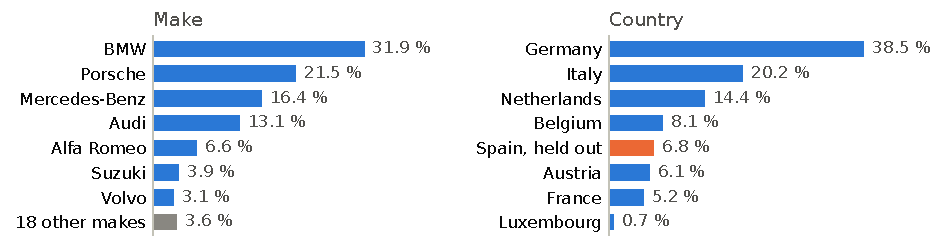
\includegraphics[width=\textwidth]{data-composition}
  \caption{The share of the 118,382 raw listings per make and per country. The Spanish listings are held out as a market the model has not seen (EDN-03); 6,079 of them remain after cleaning.}
  \label{fig:composition}
\end{figure}

The dataset card states each limitation together with what it rules out.
The target is an asking price, not a sale price.
The data is one snapshot without listing dates, so we cannot split or validate by time (EDN-32).
The raw file contains seven columns with personal data of sellers. They never reach the processed data (NFR-08), but the raw Parquet file lies on our public DVC remote, because the same data is already public on Zenodo (EDN-20).

After the scope, date, price, and deduplication rules, 105,405 of the 118,382 listings remain.
The 6,079 Spanish ones form the holdout, and we split the other 99,326 by seller in the ratio 60/10/10/20 with a pinned seed, so that no seller appears in two sets (EDN-32).
We reviewed this split strategy after training and kept it.
\Cref{tab:split} shows the result.
The validation set is used for early stopping and tuning, the calibration set is reserved for the price intervals of UC2, and the test set is what the release gate reads.

\begin{table}[ht]
  \centering\small
  \begin{tabular}{@{}lrrrrr@{}}
    \toprule
    & Train & Validation & Calibration & Test & Spanish holdout \\
    \midrule
    Rows & 61,180 & 8,992 & 9,169 & 19,985 & 6,079 \\
    Rows of the 11 supported makes & 60,378 & 8,859 & 8,987 & 19,665 & 5,979 \\
    \bottomrule
  \end{tabular}
  \caption{The split, from the dataset card. The models train and are evaluated on the rows of the supported makes.}
  \label{tab:split}
\end{table}

\subsubsection{Model card}
\label{sec:m1-model-card}
\guidance{
  \textbf{Template:} Brief description of the main points of the model card, and link to the file in the repository.\\
  Follow the Hugging Face annotated model card template \cite{hf-model-card, mitchell2019modelcards}.
  Update it in the final report once the model has changed.
}

The model card is \href{https://github.com/mlops-2627q1-mds-upc/MLOPS_Recommenditos/blob/main/docs/docs/model-card.md}{\texttt{docs/docs/model-card.md}} and follows the Hugging Face annotated template \cite{hf-model-card}.
It states at the top that no model is released yet and which of its results are measured.
Its main points:

\begin{itemize}
  \item \textbf{Model.} LightGBM on $\log(\mathrm{price})$ (EDN-02). It is compared with two baselines: B1, a Ridge regression, and B0, which predicts the median training price of cars with the same make, model, and two-year age band.
  \item \textbf{Candidate.} \texttt{lgbm-basic} uses \texttt{learning\_rate} 0.05 and \texttt{num\_leaves} 63. A grid search around these values found no better point, so we kept them (EDN-73). It is trained on its rows plus two copies of each in which optional input fields are blanked (EDN-82). Early stopping chose 1,394 trees under a ceiling of 5,000, and the model file has 8.7\,MB.
  \item \textbf{Results.} The card reports every success criterion (\cref{tab:success-criteria}), the error per segment, and the energy of each training run (\cref{sec:m3-energy}).
  \item \textbf{Who is affected by a wrong answer.} A seller acts on one number, and an estimate that is 10\,\% too low costs them money without their noticing. This is why a valuation comes with an explanation (FR-08). A buyer uses the price interval to check an offer, which is what SC-05 bounds.
  \item \textbf{Limitations.} The error on cars older than 20 years is above SC-04's bound, which we accept as a limitation of this model (EDN-62). Honda, Hyundai, Aston Martin, and Volkswagen are served but have fewer than 500 test rows each, so SC-04 does not check them.
\end{itemize}

\subsubsection{Project coordination and communication}
\label{sec:m1-coordination}
\guidance{
  \textbf{Template:} What tools have been selected, why, and how are they used?\\
  \textbf{Rubric (4 pts):} How effectively do our coordination and communication practices support collaboration and leave a useful trace of our progress?\\
  Already in place (see \texttt{docs/docs/scrum/} and \texttt{CONTRIBUTING.md}): Scrum with GitHub Issues and a GitHub Projects board, Discord for async communication, a weekly sync in the Tuesday laboratory session instead of a daily standup, a Definition of Done, working agreements, a sprint log, and issue and PR templates.
  Show the trace: board screenshot, sprint log, linked issues and PRs.
}

We work in Scrum with one-week sprints.
GitHub Issues is the backlog, a GitHub Projects board (Backlog, To Do, In Progress, In Review, Done) is the sprint board, and Discord is the team chat.
We chose GitHub for everything except chat so that an issue, its branch, its pull request, and its commit are linked to each other and the trace of our progress sits next to the code.
The board is linked on the cover.

\begin{itemize}
  \item \textbf{Ceremonies.} A sprint runs from Tuesday to Tuesday. Planning, review, and retrospective take place in the Tuesday laboratory session, the only time the whole team is in one room. We have no daily standup.
  \item \textbf{Tickets.} Every issue has an owner, a milestone label (\texttt{M1} to \texttt{M6}), and an area label such as \texttt{area:data}. Sprint~1 had no labels until its last day, so we now add them when the issue is written.
  \item \textbf{Written process.} \href{https://github.com/mlops-2627q1-mds-upc/MLOPS_Recommenditos/blob/main/docs/docs/scrum}{\texttt{docs/docs/scrum/}} and \href{https://github.com/mlops-2627q1-mds-upc/MLOPS_Recommenditos/blob/main/CONTRIBUTING.md}{\texttt{CONTRIBUTING.md}} hold the roles, the Definition of Done, and the working agreements.
  \item \textbf{Trace.} The \href{https://github.com/mlops-2627q1-mds-upc/MLOPS_Recommenditos/blob/main/docs/docs/scrum/sprints.md}{sprint log} records each sprint's goal, planning, review, and retrospective with links to its issues and pull requests (\cref{tab:sprints}). The 38 entries of \href{https://github.com/mlops-2627q1-mds-upc/MLOPS_Recommenditos/blob/main/reports/edn.md}{\texttt{reports/edn.md}} record the engineering decisions taken so far with their alternatives.
\end{itemize}

\begin{table}[ht]
  \centering\small
  \begin{tabularx}{\textwidth}{@{}llX>{\raggedright\arraybackslash}p{0.24\textwidth}@{}}
    \toprule
    Sprint & Dates (2026) & Goal & Result \\
    \midrule
    1 & 22 to 29 Sep & Coordination set up, dataset and modelling direction fixed, DVC, requirements, and the two cards started & 16 pull requests merged, 7 issues closed \\
    \addlinespace[2pt]
    2 & 29 Sep to 6 Oct & A pipeline that runs end to end on the real data, tracked in MLflow, and gated by the success criteria & 29 pull requests merged, 26 issues closed \\
    \addlinespace[2pt]
    3 & 6 to 13 Oct & Tune the model and measure its carbon emissions & in progress \\
    \bottomrule
  \end{tabularx}
  \caption{The sprints so far, from \texttt{docs/docs/scrum/sprints.md}.}
  \label{tab:sprints}
\end{table}

\paragraph{Coding agents.}
Coding agents write most of the code, under a rule in our working agreements (EDN-81).
The rule says that an independent agent with a fresh context reviews every substantive change by reproducing its claims and trying to break it, and the required checks gate the merge (\cref{tab:ci-checks} lists the nine).
A person decides the questions that belong in the EDN and is accountable for the change.
The team confirmed this wording at the laboratory session of 13 October 2026.

% Milestone 2a: project structure, code versioning and data versioning.
% Owner: @W11W11W11. The text below is a complete draft written from the
% repository's evidence. The \tbd right after the heading marks it as awaiting
% its owner's sign-off, and `make report-submit` counts it, so the draft cannot
% reach a submission unnoticed.
% Experiment tracking is the last sub-subsection of this Milestone and lives in
% sections/2-2b-experiment-tracking.tex, owned by @ulasawczuk and input at the
% bottom of this file, so that the two people writing about Milestone 2 never
% edit the same file.

\subsection{Milestone 2: Model Building -- Reproducibility}
\label{sec:m2}
\guidance{
  \textbf{Template:} Describe how the different software engineering practices and tools have been applied.\\
  EDN entries here only for reproducibility decisions that go beyond what the course prescribes.
}

\tbd{DRAFT of \crefrange{sec:m2-structure}{sec:m2-data-versioning}, owner \texttt{@W11W11W11}, to rewrite}

\subsubsection{Project structure}
\label{sec:m2-structure}
\guidance{
  \textbf{Template:} e.g.\ Cookiecutter.\\
  \textbf{Rubric (5 pts):} How well does the project structure support clarity, maintainability, and adaptation to the project's needs?\\
  We use the Cookiecutter Data Science template \cite{ccds} with uv as dependency manager.
  Justify any deviations from it (the course allows justified deviations).
}

We use the Cookiecutter Data Science template \cite{ccds} with \texttt{uv} as the dependency manager.
We changed it in five places, each for a need of this project:

\begin{itemize}
  \item \textbf{One module per pipeline stage (EDN-28).} The template's three flat modules became one module per stage, in \texttt{recommenditos/\allowbreak data/} and \texttt{recommenditos/\allowbreak modeling/}. A stage names the code it runs as its dependency, so a code change reruns only the stages it affects. Each ticket also has its own file, so several people can work on the pipeline at once.
  \item \textbf{Configuration in \texttt{params.yaml} (EDN-30).} Everything configurable is there, and \texttt{config.py} holds only paths. A changed parameter reruns the stages that read it, and \texttt{dvc params diff} shows what changed between two commits.
  \item \textbf{Two more stages than the course demo.} A tabular model needs a \texttt{features} stage. The \texttt{evaluate} stage writes the result of the release gate to a file that a person reads before promoting a model (EDN-12).
  \item \textbf{A data contract (EDN-31).} \texttt{recommenditos/schema.py} defines the columns of the raw, cleaned and processed data, and every stage checks its input and output against it (\cref{sec:m3-data-testing}).
  \item \textbf{Dependency groups (EDN-47).} \texttt{[project] dependencies} is the serving runtime only, and the pipeline and development tools are dependency groups. The API image installs only what serving needs, and a CI job checks that serving code imports nothing from a group.
\end{itemize}

\subsubsection{Code versioning}
\label{sec:m2-code-versioning}
\guidance{
  \textbf{Template:} e.g.\ GitHub Flow.\\
  \textbf{Rubric (15 pts, shared with data versioning):} How do our version control practices keep collaboration smooth and minimise mistakes?\\
  Already in place: GitHub Flow with \texttt{feature/} and \texttt{fix/} branches, branch protection on \texttt{main}, squash merge as the only merge method, Conventional Commits enforced by pre-commit and by a CI check on PR titles, pre-commit hooks (ruff, nbstripout, file hygiene).
}

We follow GitHub Flow.
\texttt{main} is the released state, every change is made on a short-lived \texttt{feature/} or \texttt{fix/} branch, and it reaches \texttt{main} through a pull request.
Tooling enforces the rules:

\begin{itemize}
  \item \textbf{Branch protection.} Nobody can push to \texttt{main} directly. A pull request can be merged once the nine required checks of \cref{tab:ci-checks} pass. No approval is required; \cref{sec:m1-coordination} describes how changes are reviewed.
  \item \textbf{Squash merge only.} \texttt{main} has one commit per pull request, so its history is a list of changes.
  \item \textbf{Conventional Commits.} A \texttt{commit-msg} hook checks them locally and a CI check verifies the pull request title, because with squash merge the title becomes the commit message.
  \item \textbf{Pre-commit hooks.} Twelve hooks run before every commit and again in CI: \texttt{ruff} as linter and formatter, \texttt{nbstripout}, \texttt{gitleaks}, and checks for whitespace, YAML and TOML syntax, merge-conflict markers, line endings and files over 1\,MB.
\end{itemize}

\begin{table}[ht]
  \centering\small
  \begin{tabularx}{\textwidth}{@{}lX@{}}
    \toprule
    Required check & What it verifies \\
    \midrule
    Lint \& format & The pre-commit hooks on every file (\cref{sec:m3-static-analysis}) \\
    Tests & The Pytest suite with coverage, on Linux (\cref{sec:m3-model-testing}) \\
    Tests (Windows) & The same suite on Windows, which one teammate develops on (EDN-75) \\
    Serving runtime & Serving code imports only the runtime dependencies (EDN-47) \\
    Requirement matrix & Every requirement due by the current milestone has its evidence (NFR-07) \\
    Notebook lint (Pynblint) & The notebook rules (\cref{sec:m3-static-analysis}) \\
    Secret scan (gitleaks) & No secret in any commit of the history (EDN-71) \\
    Build docs & The documentation site builds \\
    Conventional commit PR title & The message of the squash commit \\
    \bottomrule
  \end{tabularx}
  \caption{The nine checks that branch protection requires before a merge.}
  \label{tab:ci-checks}
\end{table}

CI first detects which areas a change touches and runs the test, documentation and report jobs only for their own area, so a documentation change does not wait for the test suite.

Three further rules prevent mistakes we made or could easily make.
The \texttt{.gitignore} ignores everything under \texttt{data/} except the \texttt{.dvc} pointer files, so a raw file with personal data cannot be committed by accident.
EDN IDs are reserved on \texttt{main} before a branch uses one, because sprint~1 assigned EDN-19 twice on parallel branches.
In the 48 hours before a presentation we merge only fixes, because every merge to \texttt{main} will deploy (NFR-13).

\subsubsection{Data versioning}
\label{sec:m2-data-versioning}
\guidance{
  \textbf{Template:} e.g.\ DVC.\\
  \textbf{Rubric:} How effectively does our data versioning strategy guarantee reproducibility and scalability?\\
  The demo uses DVC with a DagsHub remote (HTTP option) and a \texttt{dvc.yaml} pipeline \texttt{download -> preprocess -> validate -> split -> train} with code files as dependencies; commit \texttt{dvc.lock}.
  Consider a pipeline figure.
}

We version the data and the models with DVC.
The remote is the DagsHub repository of an organisation the team owns, so access follows team membership and does not depend on one member's account (EDN-19).
Each member's credentials are in \texttt{.dvc/config.local}, which Git ignores.

The pipeline is defined in \texttt{dvc.yaml} (\cref{fig:pipeline}), and the committed \texttt{dvc.lock} records the hash of every input, parameter and output.
A Git commit therefore identifies the code, the data and the parameters together, and \texttt{dvc pull} restores the artefacts that belong to it.
DVC caches every stage, so a change reruns only the stages it affects.

% figures/pipeline.pdf is drawn from dvc.yaml by figures/pipeline.sh; rerun it
% after a change to the stages.
\begin{figure}[ht]
  \centering
  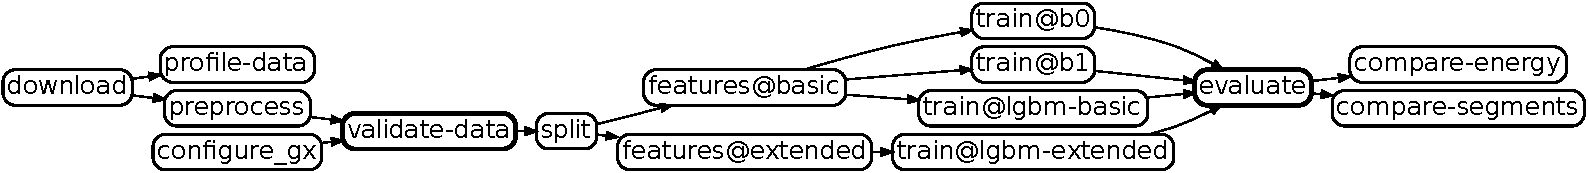
\includegraphics[width=\textwidth]{pipeline}
  \caption{The DVC pipeline as \texttt{dvc dag} draws it from \texttt{dvc.yaml}. The \texttt{features} and \texttt{train} stages exist once per model variant.}
  \label{fig:pipeline}
\end{figure}

Five properties of the pipeline go beyond the course demo:

\begin{itemize}
  \item \textbf{Raw data.} The \texttt{download} stage fetches the file from the Zenodo DOI and refuses it unless its MD5 equals the checksum Zenodo publishes (EDN-36). We keep no copy of the published CSV.
  \item \textbf{Parameters.} Each stage lists only the \texttt{params.yaml} keys it reads, and the \texttt{features} and \texttt{train} stages are generated once per variant with \texttt{foreach}. Changing the hyperparameters of one variant retrains only that variant (EDN-30).
  \item \textbf{Validation gate.} \texttt{validate-data} fails when an expectation fails, and \texttt{split} depends on its output, so no model can be trained on data that did not pass (\cref{sec:m3-data-testing}).
  \item \textbf{Synthetic data.} With \texttt{download.source} set to \texttt{synthetic}, the \texttt{download} stage generates a dataset with the same schema, and \texttt{dvc repro} runs on a clean clone without the 548.6\,MB file and without DagsHub access (EDN-33). The tests use the same generator, so no real listing is committed to Git. \texttt{metrics.json} records which source produced it.
  \item \textbf{Data contract.} Every stage checks its input and output against \texttt{schema.py} and writes only the columns it defines (EDN-31). This keeps the seven personal-data columns out of the processed data (NFR-08).
\end{itemize}

One limit is known: \texttt{dvc.lock} is reproducible only within one toolchain, because a Parquet file changes with the versions of the libraries that write it.

% Experiment tracking, owned by @ulasawczuk.
% Milestone 2b: experiment tracking. Included from sections/2-2-reproducibility.tex,
% so it appears as subsection 2.2's last sub-subsection.

\subsubsection{Experiment tracking}
\label{sec:m2-experiment-tracking}
\guidance{
  \textbf{Template:} e.g.\ MLflow.\\
  \textbf{Rubric (5 pts):} How does our experiment tracking help us and others compare, understand, and extend our results?\\
  The demo uses DagsHub as shared MLflow tracking server with credentials in \texttt{.env}.
  Show what we log (parameters, metrics, artifacts, emissions) and a comparison of runs.
  Our own starting points: one experiment \texttt{recommenditos-price} (\texttt{train.mlflow\_experiment} in \texttt{params.yaml}), one run per variant of the experiment ladder (\texttt{b0}, \texttt{b1}, \texttt{lgbm-basic}, \texttt{lgbm-extended}), and the DagsHub repository of EDN-19 as tracking server.
}

We track experiments with MLflow on the team's DagsHub repository, which is also the DVC remote (EDN-19).
The credentials are in a \texttt{.env} file that Git ignores.

\paragraph{What we track.}
The experiment \texttt{recommenditos-price} holds one run per variant of our experiment ladder (\cref{tab:runs}), a sequence of models from a simple baseline to the full model.
The ladder is defined in \texttt{params.yaml} and has four steps: \texttt{b0}, which predicts the median training price of cars with the same make, model, and two-year age band; \texttt{b1}, a Ridge regression; \texttt{lgbm-basic}, LightGBM on the 16 basic features, trained on its rows plus blanked copies of them (EDN-82); and \texttt{lgbm-extended}, LightGBM without such copies on 162 features, which add the equipment lists, the history flags, and further technical columns.
Each run logs:

\begin{itemize}
  \item the parameters of its stage and the name of its feature set;
  \item the metrics: MdAPE, the shares within $\pm$10\,\% and $\pm$20\,\%, the mean absolute error in EUR, and the success criteria;
  \item the fit time and CodeCarbon's energy and emissions figures (\cref{sec:m3-energy});
  \item the model artefact;
  \item the Git commit and the hashes of the stage's inputs, so that a run can be matched to a committed state of the pipeline (NFR-14).
\end{itemize}

\paragraph{How others can compare and extend the results.}
Each variant is its own DVC stage, so \texttt{dvc.lock} pins the code, data, and parameters behind a run, and \texttt{dvc repro train@lgbm-basic} on the same commit reproduces it.
The comparison is also committed: the \texttt{evaluate} stage writes one record per variant to \texttt{reports/metrics/} and a summary to \texttt{metrics.json}.
A pull request that changes a result shows the change in its diff, and a reader needs no account on the tracking server.
A new variant is one more entry in \texttt{params.yaml}.

\begin{table}[ht]
  \centering\small
  \begin{tabular}{@{}lrrrrrr@{}}
    \toprule
    & & \multicolumn{3}{c}{Every field given} & Required fields only & \\
    \cmidrule(lr){3-5}\cmidrule(lr){6-6}
    Run & Features & MdAPE & Within $\pm$20\,\% & MAE (EUR) & MdAPE & Fit time \\
    \midrule
    \texttt{b0} & 16 & 12.16\,\% & 70.5\,\% & 9,388 & 12.16\,\% & 0.1\,s \\
    \texttt{b1} & 16 & 9.52\,\% & 80.3\,\% & 7,499 & 10.72\,\% & 2.0\,s \\
    \texttt{lgbm-basic} & 16 & 6.73\,\% & 90.0\,\% & 4,731 & 6.86\,\% & 19.0\,s \\
    \texttt{lgbm-extended} & 162 & 6.26\,\% & 90.4\,\% & 4,651 & 10.30\,\% & 30.5\,s \\
    \bottomrule
  \end{tabular}
  \caption{The experiment ladder on the 19,665 test rows, from \texttt{reports/metrics/} and \texttt{reports/figures/energy-vs-error.csv}. The MLflow run ID of each row is in \texttt{reports/metrics/<run>.json}. Runs of 2026-10-13 on a laptop CPU.}
  \label{tab:runs}
\end{table}

\paragraph{What the comparison showed.}
\Cref{tab:runs} compares the four runs, which the \href{https://dagshub.com/recommenditos/MLOPS_Recommenditos/experiments}{experiment on DagsHub} lists as well.
The extended feature set improves the MdAPE by 0.48 percentage points when the user gives every field.
With only the fields FR-01 requires, \texttt{lgbm-extended} is at 10.30\,\%, which is 1.65 times its own full-input value and above SC-06's bound of 1.5, and it is worse than \texttt{lgbm-basic} at 6.86\,\%.
Such requests were almost absent from the training rows, and \texttt{lgbm-basic} was at 8.26\,\% on them until we trained it on blanked copies (EDN-82).
\texttt{lgbm-extended} is trained without such copies.
With them, its error on a request of the required fields fell to 7.14\,\% on the validation split, but it then lost to \texttt{lgbm-basic} on a request that gives exactly the six optional fields of the basic set.
\texttt{lgbm-extended} also takes 1.6 times as long to fit.
We therefore put \texttt{lgbm-basic} forward as the candidate (EDN-62).

The hyperparameter search is tracked separately.
Its 34 fits are runs in a second experiment, \texttt{recommenditos-price-tuning}, so they do not mix with the ladder.
The search compared \texttt{learning\_rate}, \texttt{num\_leaves}, and \texttt{min\_child\_samples} on the validation split for both LightGBM variants and found no value that is measurably better than the committed ones.
The results in \cref{tab:runs} use these values; the search was not repeated after \texttt{lgbm-basic} got its copies.


% Milestone 3: energy efficiency, static analysis, model testing, data testing.
% Owner: @michudud04. The text below is a complete draft written from the
% repository's evidence. The \tbd right after the heading marks it as awaiting
% its owner's sign-off, and `make report-submit` counts it, so the draft cannot
% reach a submission unnoticed.
\subsection{Milestone 3: Model Building -- Quality Assurance}
\label{sec:m3}
\guidance{
  \textbf{Template:} Describe how the different software engineering practices and tools have been applied.\\
  The testing strategy for code, data and model is a typical M3 EDN entry.
}

\tbd{DRAFT, owner \texttt{@michudud04}, to check and rewrite in own words}

\subsubsection{Energy efficiency awareness}
\label{sec:m3-energy}
\guidance{
  \textbf{Template:} e.g.\ CodeCarbon. Reason about the energy efficiency of your ML component.\\
  \textbf{Rubric (5 pts):} How do our energy tracking practices help us reflect on the efficiency and sustainability of our choices?\\
  The demo wraps only the \texttt{fit} call in CodeCarbon's \texttt{EmissionsTracker} and logs the result to MLflow per run.
  Go beyond reporting a number: compare models or configurations by energy versus accuracy.
}

We measure the energy of every training fit with CodeCarbon (NFR-10, EDN-69).
The tracker wraps the fit call only.
Its result goes to the MLflow run of that fit and to \texttt{reports/\allowbreak emissions/}, so the energy and the accuracy of a variant are always read together.
The \texttt{compare-energy} stage of the pipeline builds \cref{fig:energy} from these files.

The figures are estimates.
On our laptops a normal process cannot read the CPU's energy counter, so CodeCarbon estimates the power from the CPU load and a constant for the memory.
We checked the estimate once against the counter: it was about 70\,\% of the counter's reading for \texttt{b1}, \texttt{lgbm-basic} and \texttt{lgbm-extended}, and both gave the same ratio of 2.97 between the two LightGBM variants; the 0.09-second fit of \texttt{b0} is too short to compare.
We therefore use the figures to compare variants and not as absolute values.
The emissions are the energy times a fixed factor for the Spanish grid, 174.05\,g\,CO$_2$eq per kWh, so that two runs differ in emissions only through their energy and not through the location CodeCarbon detects.

\begin{table}[ht]
  \centering\small
  \begin{tabular}{@{}lrrr@{}}
    \toprule
    & Fit time & Energy & Emissions (CO$_2$eq) \\
    \midrule
    \texttt{b0} & 0.09\,s & 0.0003\,Wh & 0.06\,mg \\
    \texttt{b1} & 1.40\,s & 0.0069\,Wh & 1.19\,mg \\
    \texttt{lgbm-basic} & 9.25\,s & 0.0375\,Wh & 6.53\,mg \\
    \texttt{lgbm-extended} & 30.90\,s & 0.1119\,Wh & 19.47\,mg \\
    \midrule
    Whole ladder & 41.6\,s & 0.157\,Wh & 27.3\,mg \\
    Hyperparameter search, 34 fits, on another laptop & 391\,s & 3.61\,Wh & 628\,mg \\
    \bottomrule
  \end{tabular}
  \caption{Energy and emissions of training, as CodeCarbon estimates them (\texttt{reports/figures/energy-vs-error.csv}; the search from its MLflow runs, EDN-78).}
  \label{tab:energy}
\end{table}

\begin{figure}[ht]
  \centering
  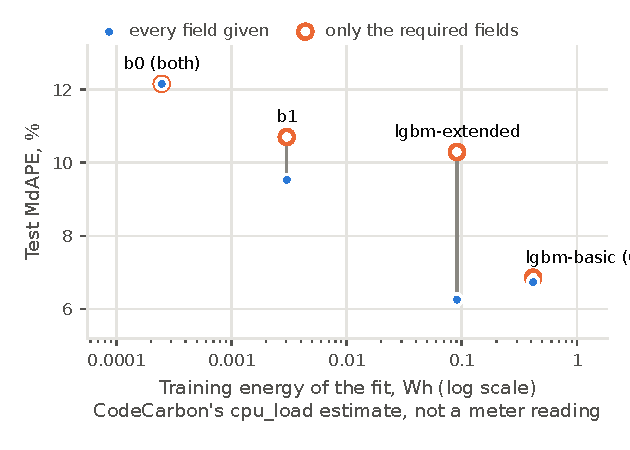
\includegraphics[width=0.66\textwidth]{energy-vs-error}
  \caption{Training energy against test error for the four variants. The blue points are requests with every field, the orange points requests with only the fields FR-01 requires.}
  \label{fig:energy}
\end{figure}

\paragraph{Feature sets.}
\texttt{lgbm-extended} needs 3.0 times the energy of \texttt{lgbm-basic} for 0.55 percentage points of MdAPE when every field is given, and it is worse when only the required fields are given (\cref{fig:energy}).
The extended features therefore do not earn their energy, which together with SC-06 is why \texttt{lgbm-basic} is the candidate (\cref{sec:m2-experiment-tracking}, EDN-62).

\paragraph{Training budget.}
The whole ladder takes 42 seconds of fitting and 0.157\,Wh, against NFR-10's budget of 15 minutes for training the chosen configuration.
By CodeCarbon's estimate the most expensive fit uses about 0.11\,Wh, so the energy of training does not limit our choices.

\paragraph{Early stopping.}
Early stopping now chooses the number of trees under a ceiling of 5,000; before, a ceiling of 1,000 ended the fit (EDN-70).
The candidate runs 1.3 times the boosting rounds for 0.02 percentage points of test MdAPE, and the fit time grows linearly with the rounds.
We accepted this so that the validation split, and not a fixed ceiling, decides the size of the model.

\paragraph{Hyperparameter search.}
The hyperparameter search ran 34 fits in 391 seconds and used 3.61\,Wh, or 628\,mg CO$_2$eq, on a second laptop (EDN-78).
That is about 23 times the whole ladder; the two were measured on different machines, so the ratio is only an order of magnitude.
The search kept the committed values.
We changed NFR-10 as a result: the 15-minute budget applies to training the chosen configuration, which every retraining pays, and a search is run and reported separately, because it is paid once per decision.

\paragraph{Serving.}
The energy of serving is not measured yet.
We will report it in Milestone~4 as an average per answer over the load test, because CodeCarbon cannot resolve a single request of a few milliseconds.

\subsubsection{Static code analysis}
\label{sec:m3-static-analysis}
\guidance{
  \textbf{Template:} e.g.\ pylint.\\
  \textbf{Rubric (10 pts, shared with model and data testing):} To what degree does our linting contribute to the overall quality and consistency of the codebase?\\
  The lab lists Pynblint (notebook and repository QA), Pylint or flake8.
  We run ruff through pre-commit and CI; the demo additionally enables Pylint rules in ruff (\texttt{PL}), which our config does too.
}

We use ruff as linter and formatter for all Python code, including the code cells of notebooks.
The rule set is \texttt{E, F, UP, B, SIM, I, PL}: pycodestyle errors, Pyflakes, pyupgrade, bugbear, simplify, import order and the Pylint rules.
The configuration is in \texttt{pyproject.toml}.

The same check runs on the same files in three places: the pre-commit hook, \texttt{make lint} and a required CI job.
On \texttt{main}, \texttt{ruff check} reports no findings and \texttt{ruff format --check} reports all 73 files as formatted.

The Pylint rules found five magic values in the command-line stubs of the template, which we removed.
We also found that \texttt{make lint} covered only \texttt{recommenditos/}, while CI linted \texttt{tests/} and \texttt{notebooks/} as well; all three now lint the same files.
Each configured exception has its reason next to it, for example the magic-value rule in \texttt{tests/}, where an assertion compares against a literal.

\paragraph{Notebooks (EDN-64, EDN-65).}
Our notebook is the exploratory analysis behind the dataset card.
It recomputes the figures of the card from the source file and fails when one does not reproduce.

Ruff checks the code in its cells, and \texttt{nbstripout} removes the outputs before every commit, which also keeps rows of the dataset with personal data out of Git.
Pynblint \cite{quaranta2022pynblint} checks the structure, for example the length of a cell and the share of Markdown cells.
We enforce 13 of its 22 rules.
The other 9 are excluded with a written reason: three read execution counts, which \texttt{nbstripout} removes, five check the repository for things CI already enforces, and one is switched off in Pynblint itself.

Pynblint exits with 0 whatever it finds, so we wrote a wrapper, \texttt{tools/notebook\_lint.py}, that reads its report and fails on any finding.
CI runs it as a required check.
The first run found five code cells over the limit of 30 lines, which we split; today it reports no findings.

\subsubsection{Model testing}
\label{sec:m3-model-testing}
\guidance{
  \textbf{Template:} e.g.\ pytest.\\
  \textbf{Rubric:} To what extent do our tests give confidence that the code and model behave as expected under different conditions?\\
  The demo tests a metric threshold on the test set and uses parametrized invariance tests.
  Optional extension listed by the demo repo: non-functional requirements (explainability with SHAP, fairness with AIF360, trustworthiness with TrustML).
}

The test suite uses Pytest and runs in CI on Linux and on Windows (EDN-75).
On \texttt{main} it has 749 tests, of which 745 pass and 4 are skipped, and it covers 98\,\% of the statements and branches of \texttt{recommenditos/}; NFR-07 requires 80\,\%.
\Cref{tab:tests} shows what the tests cover.

\begin{table}[ht]
  \centering\small
  \begin{tabularx}{\textwidth}{@{}>{\raggedright\arraybackslash}p{0.2\textwidth}X@{}}
    \toprule
    Area & What the tests check \\
    \midrule
    Pipeline stages & Every stage runs on a generated dataset in a temporary directory, without network or credentials (EDN-33). Each output satisfies its contract, the split loses no row, no seller is in two sets, and the holdout contains all Spanish listings and no others. \\
    \addlinespace[2pt]
    Edge cases & The generated dataset always contains the cases the pipeline rules exist for, such as a duplicate, a registration after the snapshot date, an unsupported make and prices outside the training range. A test of a rule therefore always finds its case in the data. \\
    \addlinespace[2pt]
    Release gate & 21 tests drive the gate with constructed models and records (NFR-01): a criterion passes and fails at its bound, and a criterion that cannot be measured blocks the gate. \\
    \addlinespace[2pt]
    Prediction & A single row gets the same prediction as the same row in a batch, and every prediction lies inside the training price range. \\
    \addlinespace[2pt]
    Tooling & The requirement matrix, the notebook lint wrapper and the EDN generator have tests of their own. \\
    \bottomrule
  \end{tabularx}
  \caption{What the test suite covers.}
  \label{tab:tests}
\end{table}

The gate tests check the logic of the gate, not the accuracy of the model.
The accuracy is measured by the \texttt{evaluate} stage on the real test split, and on every run under different conditions: in each of the 26 segments of SC-04 and in the 7 missing-field scenarios of SC-06 (\cref{tab:success-criteria}).
We have no behavioural tests of the trained model yet, such as invariance of the estimate under small changes of the input.

\paragraph{Traceability.}
A test names the requirement it verifies with the marker \texttt{@pytest.\allowbreak mark.\allowbreak req}, and a required CI job builds a requirement-to-test matrix from the markers (NFR-07).
The job fails when a requirement that is due by the current milestone has no evidence (EDN-44).
Today 67 tests carry a marker.
Of the 31 requirements, 3 are verified by a test (NFR-01, NFR-08, NFR-14), 3 are named by a test while the evidence they promise is a manual drill (NFR-06, NFR-07, NFR-10), 9 have a manual check with named evidence, and 16 have no evidence yet.
Those 16 are all due in Milestone~4 or later; the requirements due by Milestone~3 are NFR-01, 06, 07, 08, 14 and 15, and each has its evidence.

\subsubsection{Data testing}
\label{sec:m3-data-testing}
\guidance{
  \textbf{Template:} e.g.\ Great Expectations, Deepchecks.\\
  \textbf{Rubric:} How effectively does our data validation strategy anticipate and prevent potential issues in the pipeline?\\
  The demo validates raw and clean data with Great Expectations as a DVC stage and publishes Data Docs.
}

We validate the data in two layers, because they catch different problems (EDN-31).

\paragraph{Structure.}
\texttt{recommenditos/schema.py} fixes the column names, types and nullability of the raw, cleaned and processed data.
Every stage validates its input after reading and its output before writing, and it writes only the columns the contract names, which keeps the seven personal-data columns out of the processed data (NFR-08).
A violation is a bug in our code, so it fails the stage that caused it.
We wrote the contract by hand and did not use Pandera, because the contract fixes the unit of every datetime column and Pandera does not check it.

\paragraph{Values.}
Great Expectations checks the values in two DVC stages (EDN-68).
\texttt{configure\_gx} generates the expectation suites from \texttt{schema.py} and from the bounds in \texttt{params.yaml}, so each bound is defined once.
\texttt{validate-data} runs them on the raw and on the cleaned data.
\Cref{tab:validation} shows the result on the real snapshot.

\begin{table}[ht]
  \centering\small
  \begin{tabularx}{\textwidth}{@{}lrrlX@{}}
    \toprule
    Suite & Rows & Expectations & Result & What it found \\
    \midrule
    Raw & 118,382 & 103 & passed & 164 registration dates after the snapshot date (0.14\,\%, tolerated up to 1\,\%) and 3 mileage values above 1,000,000\,km (tolerated up to 0.1\,\%) \\
    \addlinespace[2pt]
    Cleaned & 105,405 & 57 & passed & No registration date after the snapshot date and no personal-data column \\
    \bottomrule
  \end{tabularx}
  \caption{Data validation on the real snapshot (\texttt{reports/data-validation/summary.json}).}
  \label{tab:validation}
\end{table}

The validation is built to stop a problem before training:

\begin{itemize}
  \item \textbf{Blocking.} A failed expectation fails \texttt{validate-data}, and \texttt{split} depends on its output, so nothing is trained on data that did not pass.
  \item \textbf{Reviewable result.} The stage writes \texttt{summary.json}, which Git tracks, so a pull request that changes the data shows what changed in the validation. It also writes the Data Docs.
  \item \textbf{Tolerances.} A registration date after the snapshot date is tolerated in up to 1\,\% of the raw rows and forbidden in the cleaned data. A new scrape with many such rows fails the raw suite and is noticed, where preprocessing alone would remove them silently (EDN-22).
  \item \textbf{Fill rates.} Both suites require the six columns that the published file fills in every row to stay filled in 99.9\,\% of the rows (EDN-77), so a column that turns empty in a new scrape fails the validation.
\end{itemize}

We dropped one planned rule after measuring it: a rule that \texttt{is\_used} and \texttt{offer\_type} agree fails for 18,108 rows of the published file, although these rows are valid (EDN-23).

\iffinalreport
  \subsection{Milestone 4: Model Deployment -- API}
\label{sec:m4}
\guidance{
  \textbf{Template:} Describe how you have deployed your model and the technologies used.
}

\subsubsection{ML-based component/system architecture}
\label{sec:m4-architecture}
\guidance{
  \textbf{Template:} Physical and logical architectures of the system, including diagrams.
  Design patterns used.
  Selection and justification of design decisions (e.g.\ cloud provider).
  The demo repo compares free tiers of AWS, Azure, GCP, Okteto, and the FIB Virtech VM (free for the semester, 4\,GB RAM, 20\,GB storage); see references/course-demos.md.\\
  \textbf{Rubric (15 pts, the largest single item):} In what ways does our system design balance clarity and justified complexity while applying suitable architectural patterns and principles?\\
  Component responsibilities and interactions are typical M4 EDN entries.
}

\tbd{logical and physical architecture with diagrams}

\paragraph{Cloud provider.}
\label{sec:m4-cloud}
We deploy on the FIB Virtech virtual machine that the course provides (EDN-17).
The course lists four free alternatives: AWS, Azure, GCP, and Okteto.

Memory decided the choice, together with the fact that the course provides the machine.
Our stack is an API container, Prometheus, Grafana, and a scheduled drift job, which does not fit into the 1\,GB and 0.6\,GB of the AWS and GCP free tiers.
Okteto offers 3\,GB and Azure between 1 and 4\,GB, depending on the instance, so neither has more memory than the 4\,GB of the FIB machine.
The FIB machine also has 20\,GB of disk and is free for the semester the project runs.
Because the course provides it, nobody needs a personal cloud account with payment details (EDN-17).

NFR-04 gives the machine a budget: the API container stays below 1\,GB of memory, the drift job runs in its own container, and the metrics and logs are capped so that the disk cannot fill up.
NFR-12 keeps the choice reversible: the system starts on a fresh machine with one command and needs no paid service, so nothing in the serving path depends on this provider.

The machine is a single host without redundancy, which is why NFR-05 asks for fast recovery and not for an uptime percentage.
Nobody on the team has access to it yet; if this is still the case at the first Milestone~4 laboratory session, we raise it with the lecturers.

\subsubsection{API design}
\label{sec:m4-api-design}
\guidance{
  \textbf{Template:} e.g.\ FastAPI.\\
  \textbf{Rubric (10 pts, shared with API testing):} To what extent do our API design and its documentation make the system robust, intuitive, and easy to adopt by others?\\
  The demo separates the FastAPI app from its Pydantic request/response schemas and relies on the generated Swagger UI (\texttt{/docs}) and ReDoc (\texttt{/redoc}).
}

\tbd{endpoints, schemas and API documentation}

\subsubsection{API testing}
\label{sec:m4-api-testing}
\guidance{
  \textbf{Template:} e.g.\ FastAPI, pytest.\\
  The demo tests the endpoints with FastAPI's \texttt{TestClient}, covering the happy path and invalid input.
}

\tbd{API tests}

  \subsection{Milestone 5: Model Deployment -- Model Packaging}
\label{sec:m5}
\guidance{
  \textbf{Template:} Describe how the different software engineering practices and tools have been applied.\\
  Containerization and CI/CD strategies are typical M5 EDN entries.
}

\subsubsection{Container and orchestration}
\label{sec:m5-containers}
\guidance{
  \textbf{Template:} e.g.\ Docker, Docker Compose.\\
  \textbf{Rubric (5 pts):} In what ways does our containerization approach guarantee portability, modularity, consistency, and efficiency across environments?\\
  The demo Dockerfile is minimal (pip + requirements.txt); building from \texttt{uv.lock} with a multi-stage, slim, non-root image is an easy way to go beyond it.
}

\tbd{container images and orchestration}

\subsubsection{CI/CD}
\label{sec:m5-cicd}
\guidance{
  \textbf{Template:} e.g.\ GitHub Actions.\\
  \textbf{Rubric (10 pts):} What aspects of our CI/CD pipeline demonstrate that automation and collaboration are fully integrated into our process?\\
  Already in place: GitHub Actions running pre-commit, tests, the docs build, this report's build, and a Conventional Commits check on PR titles, with path filters that skip jobs unrelated to a change.
}

\tbd{CI/CD pipeline}

  \subsection{Milestone 6: Monitoring}
\label{sec:m6}
\guidance{
  \textbf{Template:} Describe how the different software engineering practices and tools have been applied.
  (The course template labels this section \enquote{Milestone 5}; it is Milestone~6.)\\
  Monitoring of the running system, data, and model (degradation, drift, anomalies) is a typical M6 EDN entry.
}

\subsubsection{Resource monitoring}
\label{sec:m6-resources}
\guidance{
  \textbf{Template:} e.g.\ Grafana, Prometheus.\\
  \textbf{Rubric (5 pts):} To what extent does our monitoring anticipate real-world challenges and provide actionable insights into system performance?\\
  The lab schedule also lists Better Uptime for availability checks.
}

\tbd{resource monitoring setup and dashboards}

\subsubsection{Model performance}
\label{sec:m6-model-performance}
\guidance{
  \textbf{Template:} e.g.\ Alibi Detect.\\
  \textbf{Rubric (5 pts):} To what extent does our monitoring provide timely, actionable signals about data changes, model performance degradation, and user impact?
}

\tbd{drift detection and model performance monitoring}

\subsubsection{Cycle: feedback loops and retraining}
\label{sec:m6-feedback}
\guidance{
  \textbf{Template:} Description of all the stages of the system pipeline, and how they are connected.
  Explain how the pipeline can be used to automate the retraining process.
}

\tbd{end-to-end pipeline and automated retraining}

  % Self-evaluation / retrospective. Only built into the final report
% (report.tex inputs this file inside \iffinalreport), so it costs the initial
% delivery no pages; it is drafted now so the team has something to react to.
% Owner: the whole team, in the laboratory session. Everything below is a draft
% assembled from the sprint records in docs/docs/scrum/sprints.md so that the
% team has a starting point, not finished text. The \tbd right after the heading
% says so in the PDF as well, and `make report-submit` counts it, so the draft
% cannot reach a submission unnoticed.
\section{Self-evaluation of the project (retrospective)}
\label{sec:retrospective}
\guidance{
  \textbf{Template:} To do in the final deliverable (this section only appears in the final report build).
  Explain the main challenges, barriers, and opportunities we encountered.
  Describe what we learned and what we would do differently.
  Explain which concepts we used from which other courses.
}

\tbd{DRAFT for the whole team to confirm and extend in the laboratory session. Everything below is assembled from the sprint records and retrospective notes in \texttt{docs/docs/scrum/sprints.md}, which cover sprint~1 and the start of sprint~2 only. It is a starting point for the retrospective, not its outcome: the team confirms, corrects, and extends it together, and each member supplies their own part of \cref{sec:retro-courses}.}

\subsection{Challenges, barriers, and opportunities}
\label{sec:retro-challenges}

\paragraph{The pipeline is sequential, and five people are not.}
The single largest barrier was structural rather than technical.
Download feeds preprocessing, which feeds validation, the split, the features, the training, and the evaluation, so for as long as none of the contracts between the stages existed, only one person could work on the pipeline at a time.
Sprint~1 showed what that costs: seven pull requests were open simultaneously, two of them with merge conflicts, and nothing could be built on the data contract while its own pull request was open.
Sprint~2 was cut around the barrier instead of around the milestones, by landing the shared contracts first: one ticket delivered every DVC stage as a running stub, \texttt{params.yaml}, the schema contract, and a synthetic fixture, and it unblocked eight tickets at once.
The same cut gave each remaining ticket its own files, which is why one owner per file also became the rule for this report.

\paragraph{Evidence that stops being true.}
Several decisions were taken on measurements committed to the repository, and then a later scope decision changed the data under them.
When we dropped the listings registered after the snapshot date, the committed analysis outputs behind two EDN entries no longer reproduced, and re-running them changed one requirement's configuration from passing to failing.
Three successive written forms of the drift requirement were refuted by measurement in this way, the last because the detector's significance level and the requirement's false-alarm promise were the same number by construction and nobody had noticed.
The opportunity in it is the one the course is about: a requirement that has been measured is worth more than one that has been agreed, and the cost of finding out late is a re-run rather than a rewrite.

\paragraph{Contradictions between our own documents.}
Two of them surfaced in review rather than in use: the requirements declared the raw data would never be re-hosted while the project brief still called that question open and the data-versioning page showed the opposite example; and the requirements treated the deployment target as settled in eight places while the brief listed it as open.
Each was a decision made by writing rather than by deciding.

\paragraph{Premises nobody had checked.}
Two decisions were reached on a premise that turned out to be false, both within the same week.
The raw-data decision rested on the DagsHub repository being private, which it was not; anonymous access is refused for public and private repositories alike, so the observation behind it had no discriminating power.
And the choice of which DagsHub repository to use was taken on measurements that were all correct, about a repository belonging to somebody who is not on the team.
In both cases the check that settled it was one API call and was available before the decision rather than after it.

\paragraph{An uneven distribution of work in sprint~1, and what we changed.}
The sprint~1 retrospective records that in that first sprint almost every commit on \texttt{main} came from one person.
Because the laboratory grade carries an individual factor based on contributions, the team treated that as a finding to act on rather than as an observation, and turned it into an action item in the same session: every member owns at least one pipeline stage and writes the report section for the practice they built.
The sprint~2 plan is cut that way, with the download and preprocess stages, the split and features stages, the training stage and its emissions tracking, the Great Expectations suites, and the evaluate stage each assigned to a different member, and the section ownership of this report follows the same rule of one owner per file.
This is a statement about sprint~1 and the correction it produced, not about the delivery as a whole; whether the correction held is what the sprints after it show.
\tbd{the team's own account of how the distribution developed over sprints~2 and~3, and whether the action item worked}

\paragraph{External dependencies we do not control.}
Nobody on the team has access to the virtual machine the deployment is designed for, and that has a trigger rather than an owner: if it is still true at the Milestone~4a laboratory, we raise it with the teachers.
The dataset's licence contradicts itself on its own upstream record, and we chose to report both readings rather than wait for the author.
The data itself is the standing limitation: four premium brands are 82.9\,\% of it, which is why the scope had to become an explicit rule and why part of the quality gate is blind to four of the eleven supported makes.

\paragraph{Opportunities we took.}
Holding a whole country out of training turned the monitoring milestone from a simulation into a measurement, because every held-out listing carries a real price.
Making the data source a parameter meant a synthetic fixture could unblock five people without anyone being able to ship a model trained on fabricated data unnoticed.
And writing the decisions down as they were taken, with their alternatives, meant the report can cite reasoning rather than reconstruct it.

\tbd{the team's additions for Milestones 4 to 6: what the deployment, the packaging, and the monitoring turned out to cost, and which of the risks above actually materialised}

\subsection{Lessons learned and what we would do differently}
\label{sec:retro-lessons}

\paragraph{Land the contracts before the work that depends on them.}
The single change that made the project move was landing the schema, the parameters, and the fixture as one ticket before anybody started on a stage.
We would do that first next time rather than after a sprint of pull requests blocking each other.

\paragraph{Measure a requirement before committing to it, not after.}
Every requirement that made a claim about the data rather than about the system was wrong on first writing.
Writing the acceptance criterion as something a script can run, and then running it, is what caught that; doing it after the requirement was agreed is what made it expensive.

\paragraph{State the premise a decision rests on, and verify it.}
Both decisions that had to be withdrawn were withdrawn for a premise, not for a measurement.
The rule we now follow is to name the premise in the decision record and check it before recording, because the check is nearly always cheaper than the retraction.

\paragraph{A check has to sit where the value is consumed.}
The synthetic fixture's first version was wrong in a way its own tests could not see, because the tests asserted that each edge case existed in the raw frame while the stages consume them after preprocessing, which deleted most of them.
Asserting that each case survives the rules, rather than that it exists, is the form of the test that has signal.
This also became the rule for working with coding agents: a ticket handed to an agent needs a local oracle, and an agent's claim decides nothing until it has been checked at the point the value is used.

\paragraph{Make the process trace a by-product of the work.}
Labels, milestones, and owners assigned when a ticket is written cost nothing; assigned at the sprint review they cost a reconstruction from the git history, and six tickets of sprint~1 never got them at all.
The same applies to the ceremonies: holding them in the one session where the whole team is present is worth more than holding them on the day a document happened to name.

\paragraph{Reserve shared identifiers centrally.}
Two branches handed out the same EDN identifier, and since the report cites those identifiers they cannot be renumbered afterwards without breaking the citation.
Reserving the number on \texttt{main} before opening the branch is one line of process for a class of merge conflict that cannot be resolved cheaply.

\tbd{the team's additions after Milestones 4 to 6, and the one or two changes each member would make to how we worked}

\subsection{Concepts from other courses}
\label{sec:retro-courses}

\tbd{which concepts from which other Master courses each of us used, named per member. Nothing in the repository records this, so it has to come from the team: candidates to prompt the discussion are software engineering and testing, software architecture, statistics and statistical inference for the drift tests and the conformal intervals, machine learning for the model family and the evaluation protocol, data engineering for the pipeline, and project management for the Scrum process.}

\fi

{\small\setlength{\bibitemsep}{0pt}\printbibliography[heading=bibintoc]}

% Logged for build.sh: the room left on the last page, which is how much the
% sections can still grow before the report gains a page.
\par
\typeout{Report: space left on the last page:
  \the\dimexpr\pagegoal-\pagetotal\relax\space
  (about \the\numexpr\dimexpr\pagegoal-\pagetotal\relax/\baselineskip\relax\space lines)}
% The page limit counts the report, not the appendix.
\clearpage
\typeout{Report: pages before the appendix: \the\ReadonlyShipoutCounter}

\appendix
% A divider page, so the reader sees where the report ends and the appendices begin.
\appendixdivider
\appendixpdf{Engineering Decision Notebook}{build/\EdnJob.pdf}{app:edn}

\end{document}
